\chapter{Detección de biomarcadores en cáncer de hígado y colon-recto}

\section{Objetivos}

El objetivo general consiste en intentar predecir en base a pocos genes si una enfermedad padece o no cáncer de hígado, o cáncer de colon-recto. Para ello se usarán distintas técnicas de selección de características: mRMR, RF y DA, así como varios algoritmos de clasificación: SVM, RF y kNN.

\section{Metodología}

\subsection{Fuente de datos}

La fuente de los datos es GDC (Genomic Data Commons) Portal, una plataforma web sobre cáncer del Instituto Nacional del Cáncer de Estados Unidos (\textit{National Cancer Institute}) \cite{GDCPortal, NationalCancerInstitute}. GDC Portal fue desarrollado por el Instituto Nacional del Cáncer de Estados Unidos, la Universidad de Chicago, el Instituto de Ontario para la Investigación del Cáncer y la empresa \textit{Leidos Biomedical Research}, y su principal fortaleza reside en la integración y armonización de diversas fuentes heterogéneas, creando así un sistema de información amplio y robusto \cite{Grossman2016}. \\

\newpage
\textbf{\textcolor{red}{Figura XX}}. Diagrama de funcionalidad y utilidad de GDC. Extraído de Grossman et al. \cite{Grossman2016}.
\begin{center}
	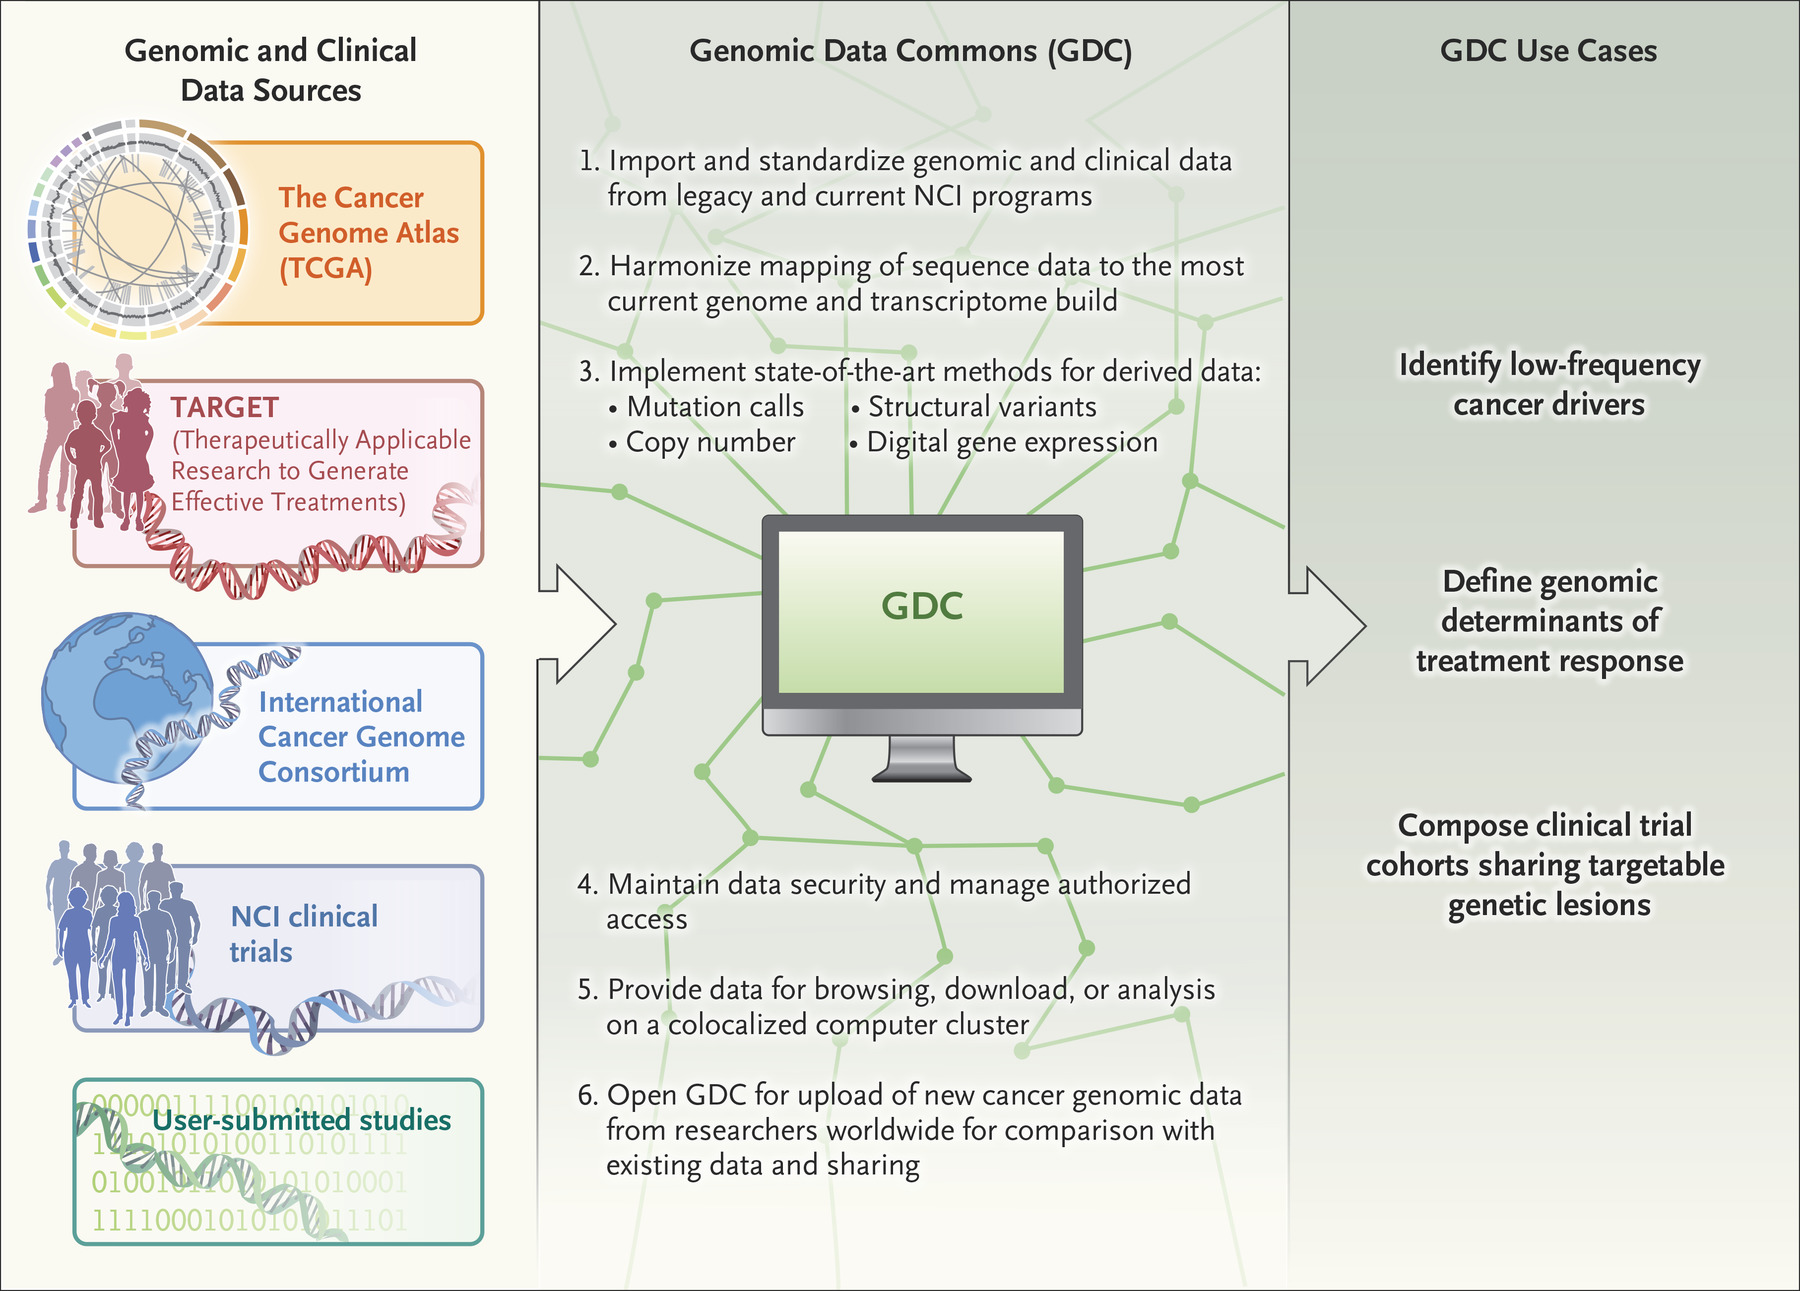
\includegraphics[width=1\textwidth]{figuras/funcionamiento_gdc.jpeg} \\
\end{center}

GDC Portal, a día 22 de Junio, contenía información sobre unos 84.000 casos, 23.000 genes y más de 3 millones de mutaciones de genes \cite{GDCPortal}. Algunos de estos datos son abiertos, mientras que para otros es necesario solicitar acceso. Los datos de los que dispone son muy variados, y se pueden distinguir en tres grandes categorías:

\begin{itemize}
	\item Información clínica, como la edad del sujeto, su sexo o el estadio del cáncer del que ha sido diagnosticado.
	\item Información genética y transcriptómica proveniente de diversos proyectos de investigación.
	\item Imágenes de tejidos tumorales y sanos.
\end{itemize} 

Para el presente trabajo se han descargado de GDC Portal todos los datos que cumplen las siguientes condiciones:

\begin{itemize}
	\item Son datos transcriptómicos del programa Cancer Genoma Atlas (TCGA), dirigido por dos organismos estadounidenses: el Instituto Nacional del Cáncer (NCI) y el Instituto Nacional para la Investigación del Genoma Humano (NHGRI) \cite{NationalCancerInstitutea}. 
	\item Contienen información sobre tumores o tejidos sanos de cáncer de hígado, o colon-recto. Se han excluido metástasis en hígado y tumores recurrentes.
	\item El tipo de estrategia experimental es RNA-Seq, y el tipo de flujo de trabajo es HTSeq - Counts.
\end{itemize}

Para cáncer de hígado, se han descargado datos sobre 462 pacientes, de los cuales 404 tenían cáncer de hígado (87,4\%) y 58 no tenían cáncer de hígado (12,6\%).

\textcolor{red}{Para cáncer de colon-recto...}

\subsection{Análisis}

Para el análisis se ha utilizado el software estadístico \texttt{R} \cite{R} y el paquete \texttt{KnowSeq} (v.1.1.19), librería que ha sido desarrollada por los tutores del presente trabajo, y en la que el autor ha contribuido con pequeñas actualizaciones \cite{KnowSeq}. El paquete está además disponible en Bioconductor, la plataforma de código abierto en R más relevante para el análisis de datos de genómica y transcriptómica \cite{Gentleman2004}.\\

Para asegurar la reproducibilidad de los análisis, en el \nameref{anexo1} (caja 1) se muestran todos los paquetes utilizados y sus versiones, como resultado de ejecutar \texttt{devtools::session\_info()}.\\

Todo el código de los análisis está disponible en el repositorio de GitHub del presente Trabajo Fin de Máster \cite{Redondo-Sanchez2020}. En el \nameref{anexo1} se muestra también el código de los análisis realizados para cáncer de hígado.

\section{Resultados: cáncer de hígado}

\subsection{Características clínicas de los pacientes}

\textcolor{red}{Tablas descriptivas de edad, sexo, raza, etnia, edad, estadio y estado vital.}

\subsection{Entrenamiento de modelo}

\subsection{Validación en test}

\section{Resultados: cáncer de colon-recto}

\textcolor{red}{Completar una vez esté depurado el análisis de cáncer de hígado}

\section{Conclusiones}

\textcolor{red}{Interpretar resultados con cautela: ver pág. 65 de \cite{CastilloSecilla2020} (referencias 77-79).}\\
